\documentclass[10pt]{article}
\usepackage{amsmath}
\usepackage{amssymb}
\usepackage[left=1in,right=1in,top=1in,bottom=1in]{geometry}
\usepackage{fancyhdr}
\pagestyle{fancy}
\usepackage{enumerate}
\usepackage{mathtools}
\usepackage{bbm}
\usepackage{amsfonts}


\newcommand{\defeq}{\vcentcolon=}
\newcommand{\eqdef}{=\vcentcolon}
\newcommand{\R}{\mathbb{R}}
\newcommand{\E}{\mathbb{E}}
\newcommand{\1}{\mathbbm{1}}
\newcommand{\V}{\text{Var}}
\newcommand{\C}{\text{Cov}}

\lhead{Data Mining}
\chead{\textbf{Homework 2}}
\rhead{Solutions}

\begin{document}
\begin{enumerate}
%% PROBLEM 1
\item 

\begin{enumerate}[(a)]
\item We can derive the result as follows
\begin{align*}
\text{df}(\hat y) &= \frac{1}{\sigma^2} \sum_{i=1}^n \C(\hat{y}_i,y_i) & \\
&= \frac{1}{\sigma^2} \text{tr}\left[\C(\hat{y},y)\right] & \C(\hat{y}_i,y_i)=\C(\hat{y},y)_{i,i}\\
&= \frac{1}{\sigma^2} \text{tr}\left[\C(Hy,y)\right] & \hat{y} = Hy\\
&= \frac{1}{\sigma^2} \text{tr}\left[H\C(y,y)\right] & \C(Ax,y) = A\C(x,y) \text{ in general}\\
&= \frac{1}{\sigma^2} \text{tr}\left[\sigma^2 H\right] & \C(y,y) = \V(y) = \sigma^2 I\\
&= \text{tr}(H) & \text{tr}(cX) = c\cdot\text{tr}(X)\\
&= \text{rank}(X) &\\
&= p &
\end{align*}
The last two lines follow from the fact that $H$ is a projection onto the column space of $X$. In general, the trace of a projection is equal to the dimension of the space onto which it projects. In this case the dimension is the rank of $X$, which is the number of predictors, $p$.
\item As shown in Homework 1 Problem 3, ridge regression is equivalent to linear regression with a modified hat matrix $H_{\text{ridge}} = X(X^TX+\lambda I)^{-1}X^T$. We can plug this in to the previous derivation:
\begin{align*}
\text{df}(\hat{y}_\text{ridge}) &= \text{tr}(H_\text{ridge}) \\
&=  \text{tr}\left[ X(X^TX+\lambda I)^{-1}X^T\right]
\end{align*}
Note that $H_\text{ridge}$ is not a projection matrix if $\lambda \neq 0$.
\end{enumerate}


%% PROBLEM 3
\stepcounter{enumi}
\item
\begin{enumerate}[(a)]
\item The following plot shows fitted curves selected by 10-fold cross validation.
\begin{center}
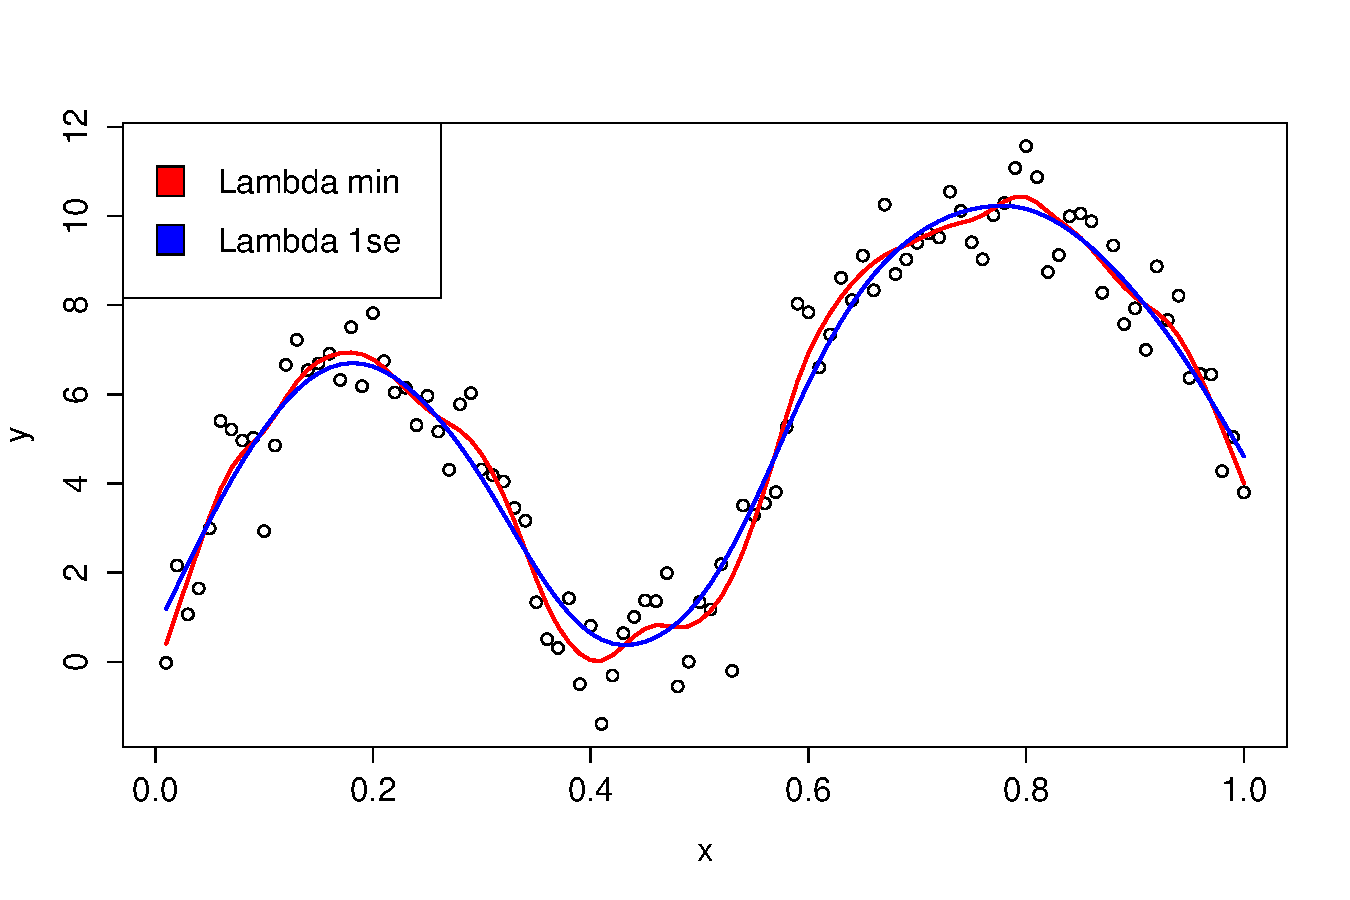
\includegraphics[width=5in]{prob3_a_1.pdf}
\end{center}
The curves are very similar, but the model with $\lambda_{1\text{se}}$ looks like it fits better. The one standard error rule creates a much smoother curve.
\item The following plot shows curves fitted with 5-fold cross validation, with each fold sequential rather than using alternating points.
\begin{center}
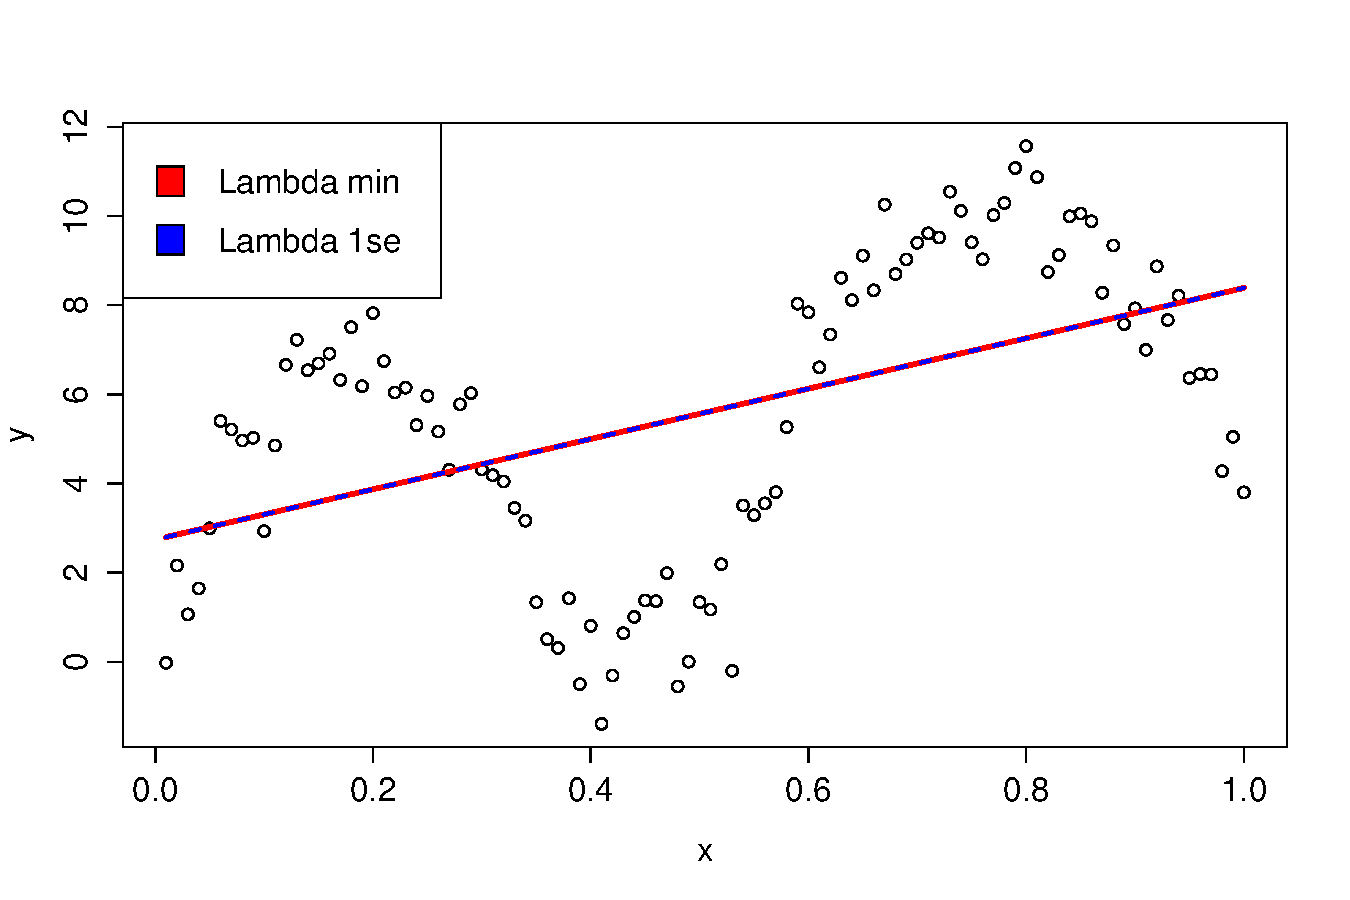
\includegraphics[width=5in]{prob3_b_1.pdf}
\end{center}
In this case cross validation chooses the simplest possible model. This is likely because models with more degrees of freedom extrapolate poorly on excluded segments of the data.

Alternatively, if we use 10 fold CV we get the following plot
\begin{center}
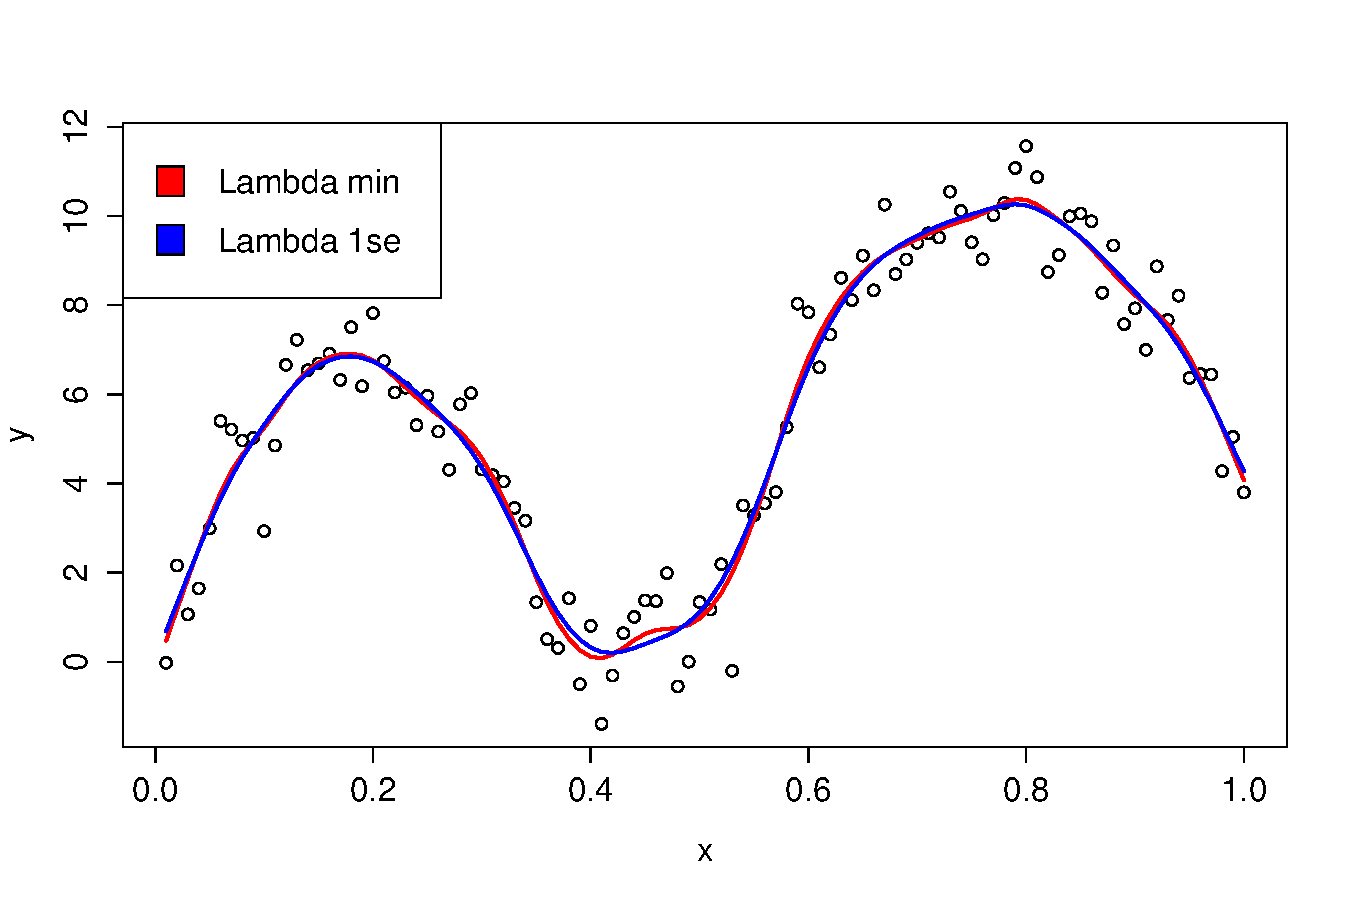
\includegraphics[width=5in]{prob3_b_2.pdf}
\end{center}
\item The following plot compares the result of leave-one-out cross validation with the shortcut formula.
\begin{center}
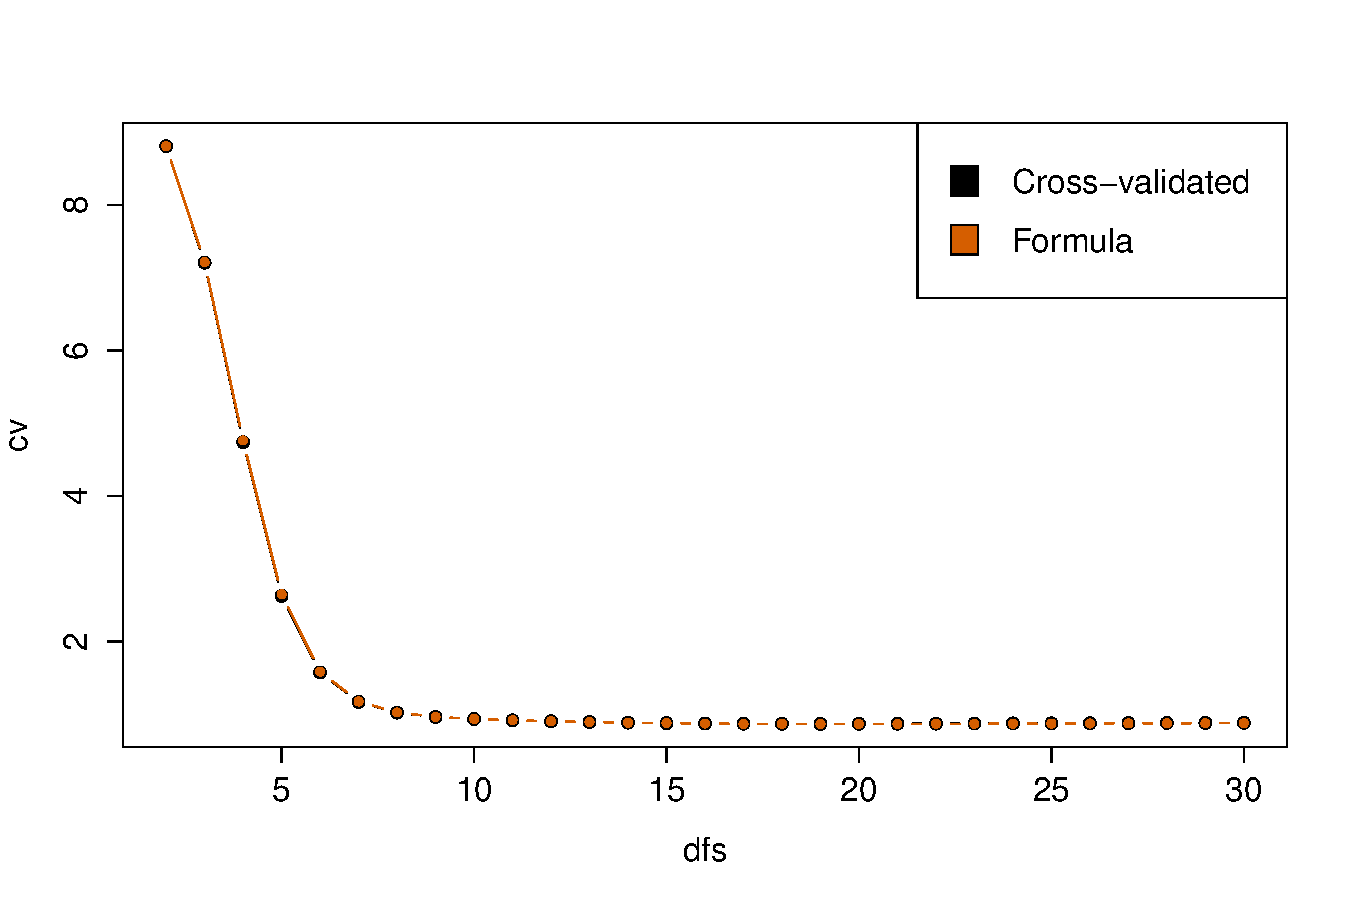
\includegraphics[width=5in]{prob3_c_1.pdf}
\end{center}
The plot shows that the values are nearly the same over the various degrees of freedom, as should be expected from Problem 4.
\end{enumerate}

\subsubsection*{Code}
{\scriptsize
\begin{verbatim}
#Load the data (appears in variable y in the workspace)
load(file="splines.Rdata")
#100 points uniformly spaced from 0 to 1
n = 100
x = 1:n/n

K = 5 #Number of folds (5 or 10 for parts A and B, 100 for part C)

#Generate a list with index vectors for each fold
folds = vector(mode="list",length=K)
for (k in 1:K) {
  #Choose folds to alternate sequentially
  
  #Folds for parts A and C
  #folds[[k]] = seq(k,n,by=K) 
  
  #Folds for part B:
  #folds[[k]] = ((k-1)*(n/K)+1):(k*n/K)
}

dfs = 2:30#Range of degrees of freedom (similar to lambda)
ndfs = length(dfs)

#Store the error at every point for every degree of freedom.
#This makes sense, because each point only gets estimated once,
#when its fold is held out
errs = matrix(0,n,ndfs)

#Run CV
for (k in 1:K) {
  #Build the test and training data sets corresponding to the kth fold
  #Variables ending in .tr are for training
  #Variables ending in .val are for validation (the held out fold)
  i.tr = unlist(folds[-k])
  i.val = folds[[k]]
  x.tr = x[i.tr]    
  y.tr = y[i.tr]   
  x.val = x[i.val] 
  y.val = y[i.val]
  
  #Fit and evaluate a spline on this fold at each degree of freedom being considered
  for (j in 1:ndfs) {
    a = smooth.spline(x.tr,y.tr,df=dfs[j])
    yhat = predict(a,x=x.val)$y
    errs[i.val,j] = (yhat-y.val)^2
  }
}

predict(a,x=x.val)$y
predict(a,newx=x.val)$y

#Average cv error across folds for each degree of freedom
cv = colMeans(errs)

#Compute the standard error across the folds for the cv estimate
errs0 = matrix(0,K,ndfs)#Stores the average error for each fold (so we can take variance)
for (k in 1:K) {
  # if using folds < n
  # errs0[k,] = colMeans(errs[folds[[k]],])
  # if using LOOCV
  # errs0[k,] = colMeans(matrix(errs[folds[[k]],],nrow=1))
}
se = apply(errs0,2,sd)/sqrt(K)

# Usual rule
i1 = which.min(cv)
# One standard error rule---note the min!
i2 = min(which(cv<=cv[i1]+se[i1]))

#Plot the cv curve
plot(dfs,cv,type="l",ylim=range(c(cv-se,cv+se)))
points(dfs,cv,pch=20)
lines(dfs,cv-se,lty=3)
lines(dfs,cv+se,lty=3)
abline(v=dfs[i1],col="red",lty=2)
abline(v=dfs[i2],col="blue",lty=2)
legend('top',fill=c('red','blue'),legend=c("Lambda min","Lambda 1se"))

#Form estimates for lambda_min and lambda_1se
yhat1 = smooth.spline(x,y,df=dfs[i1])$y
yhat2 = smooth.spline(x,y,df=dfs[i2])$y

#Plot splines for lambda_min and lambda_1se
plot(x,y)
lines(x,yhat1,col="red",lwd=2)
lines(x,yhat2,col="blue",lwd=2)
legend('topleft',fill=c('red','blue'),legend=c("Lambda min","Lambda 1se"))

#Part C: You can eventually put your code down here to get the S_ii elements and compare your LOOCV to the equation from the homework

#Computing LOOCV using the closed form formula (Part C)
closed_form = numeric(ndfs)
for(j in 1:ndfs){
  a = smooth.spline(x,y,df=dfs[j])
  yhat = predict(a,x=x)$y
  Sii = a$lev
  closed_form[j] = mean(((y-yhat)/(1-Sii))^2)
}
plot(dfs,cv,type='b',pch=19)
lines(dfs,closed_form,type='b',col="#D55E00",pch=20)
legend('topright',legend=c("Cross-validated","Formula"),fill=c("black","#D55E00"))
#The two match quite closely!
\end{verbatim}
}


%% PROBLEM 5
\stepcounter{enumi}
\item
\begin{enumerate}[(a)]
\item The dimension of the original feature space is 256, while dimension of the transformed space is 2. The following plot shows the data in the transformed space:
\begin{center}
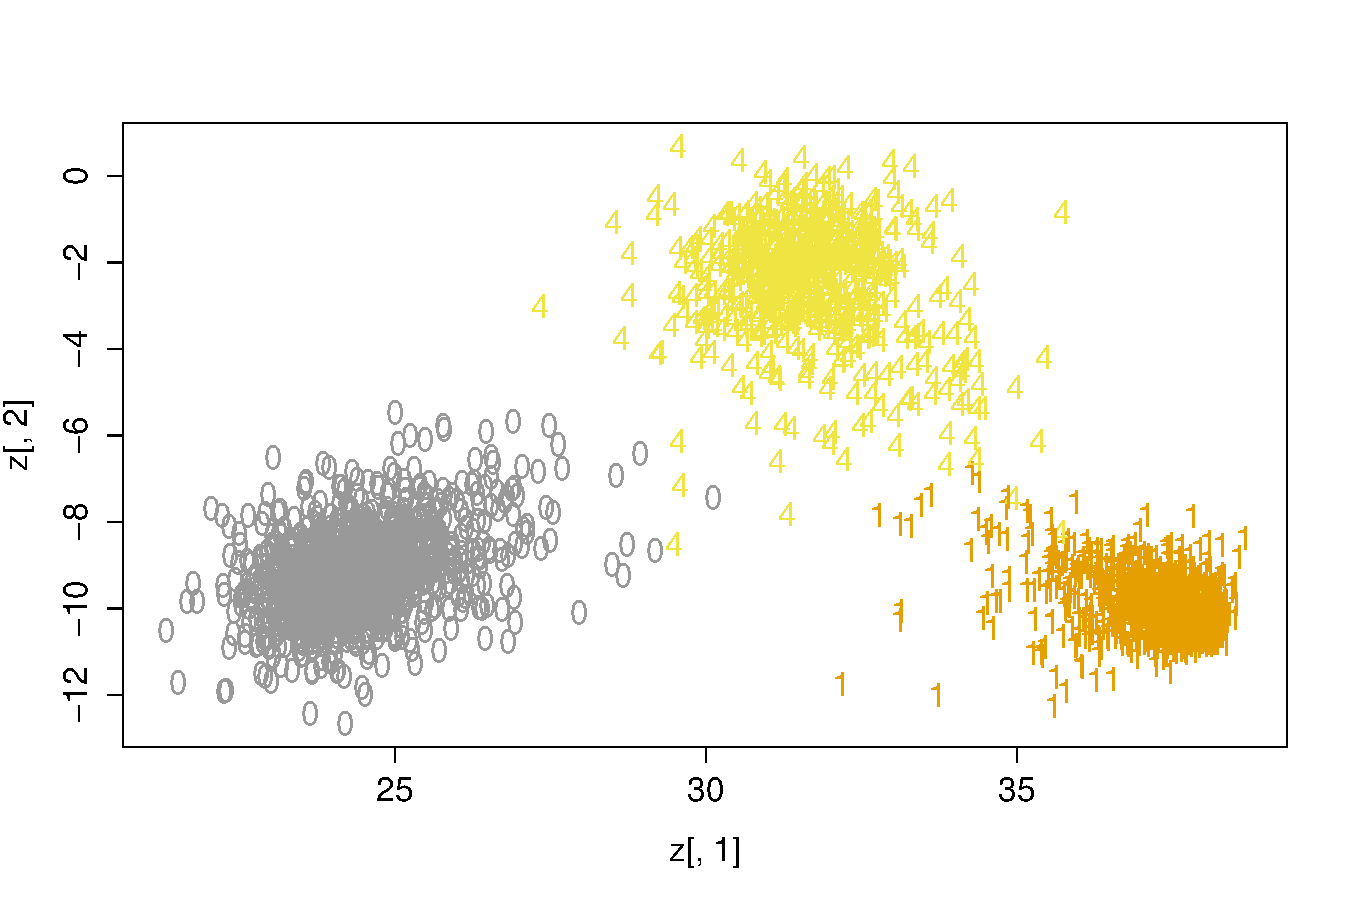
\includegraphics[width=3.5in]{prob5_a_1.pdf}
\end{center}

\stepcounter{enumii}
\item The misclassification rate is $2.07\%$. See code.
\item We replot the data with misclassified points labeled.

\begin{center}
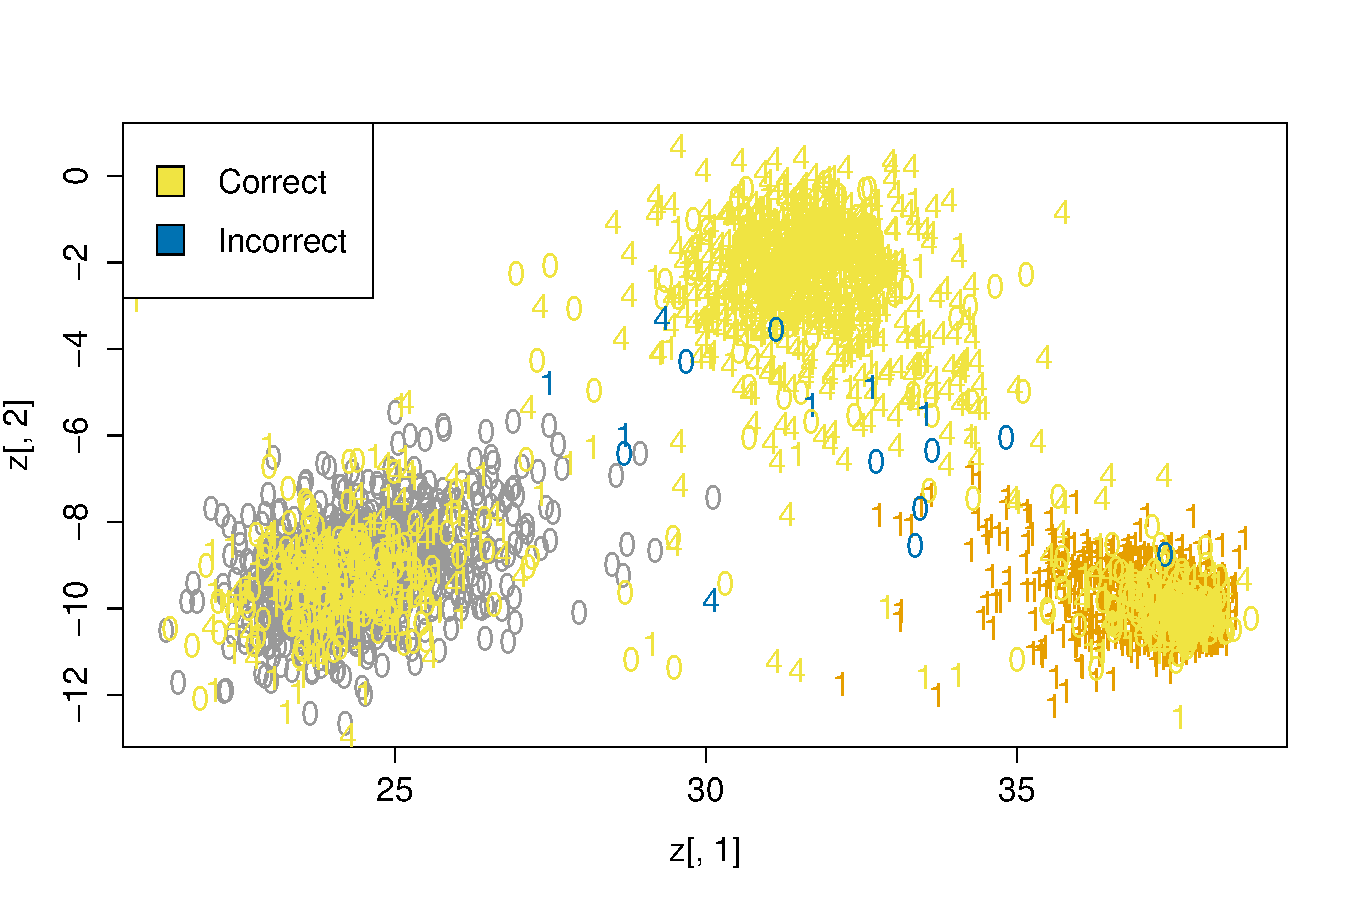
\includegraphics[width=3.5in]{prob5_d_1.pdf}
\end{center}
Some of the misclassified points are shown below.
\begin{center}
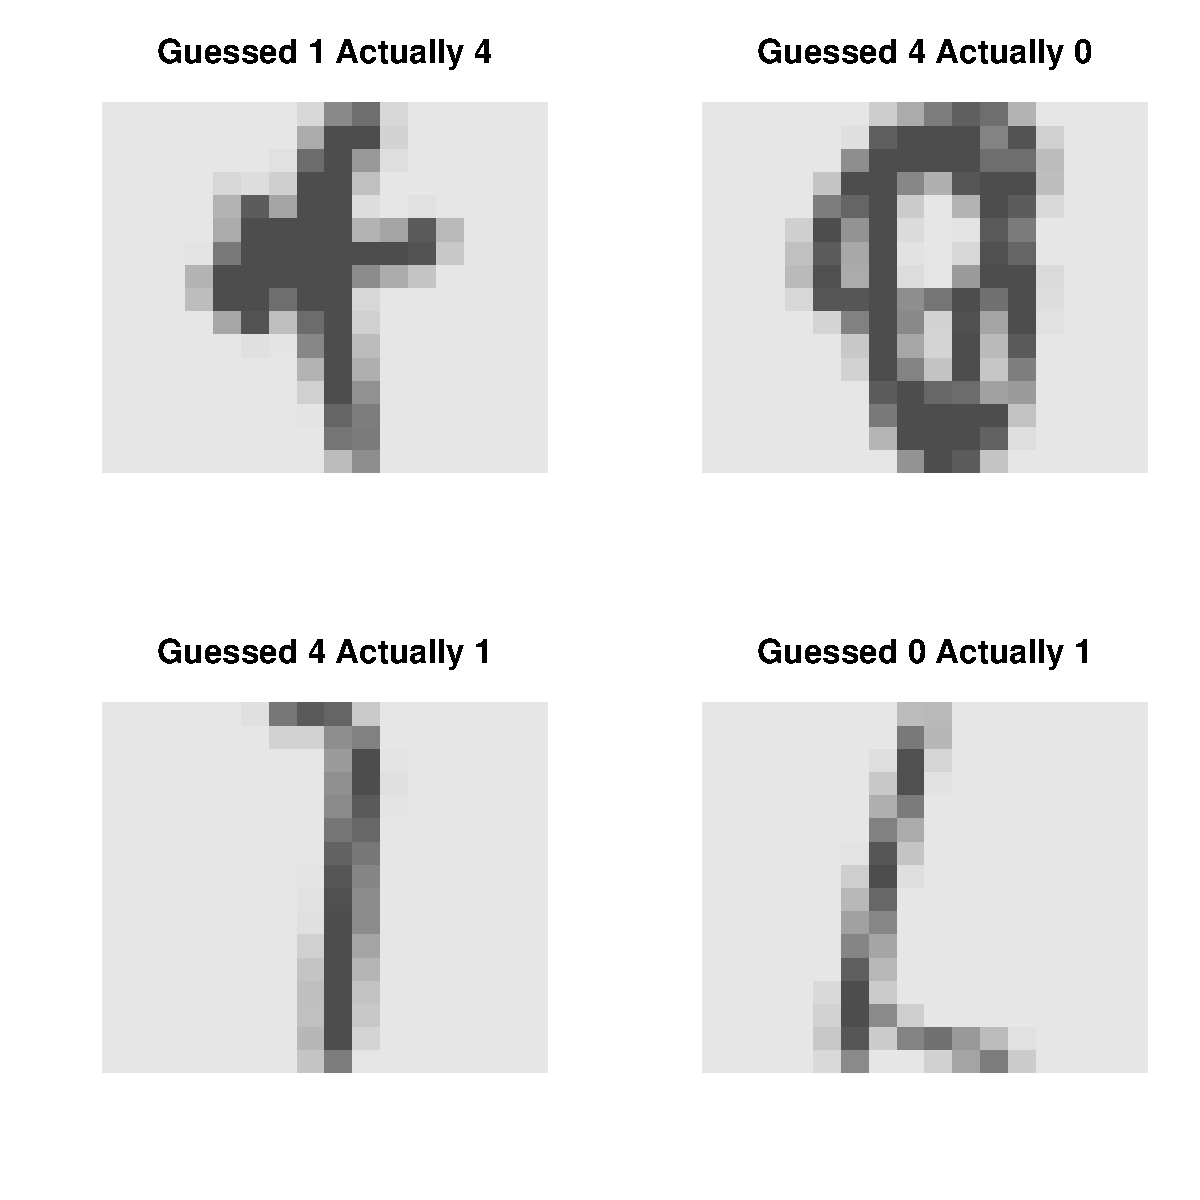
\includegraphics[width=3.5in]{prob5_d_2.pdf}
\end{center}
Going clockwise from the top left, the first and fourth misclassified examples are easy to classify by eye so you would hope the algorithm could correctly predict them. The second and third misclassified examples, on the other hand, are very ambiguous.
\end{enumerate}
\subsubsection*{Code}
{\scriptsize
\begin{verbatim}
load('zip.014.Rdata')

#A
library(MASS)
a = lda(x.014.tr,y.014.tr)
z = x.014.tr%*%a$scaling

#original dimension
ncol(x.014.tr)
#new dimension
ncol(z)

cbPalette <- c("#999999", "#E69F00", "#56B4E9", "#009E73", "#F0E442", "#0072B2", "#D55E00", "#CC79A7")#I like these colors more
plot(z[,1],z[,2],pch=as.character(y.014.tr),col=cbPalette[y.014.tr+1])

yhat = predict(a,newdata = x.014.te)$class
#Misclassification rate
mean(yhat!=y.014.te)

#Transform the test points into the same space as the training points
z.te = x.014.te%*%a$scaling

plot(z[,1],z[,2],pch=as.character(y.014.tr),col=cbPalette[y.014.tr+1])
points(z.te[,1],z.te[,2],pch=as.character(y.014.tr),col=cbPalette[5+(yhat!=y.014.te)])
legend('topleft',legend=c("Correct","Incorrect"),fill=c("#F0E442", "#0072B2"))

plot.digit = function(x,zlim=c(-1,1)) {
  cols = gray.colors(100)[100:1]
  image(matrix(x,nrow=16)[,16:1],col=cols,
        zlim=zlim,axes=FALSE)  
}
idx = which(yhat != y.014.te)
par(mfrow=c(2,2))
for(i in 1:4){
  plot.digit(x.014.te[idx[i],])
  title(paste("Guessed",yhat[idx[i]],"Actually",y.014.te[idx[i]]))
}
\end{verbatim}
}
\end{enumerate}

\end{document}
